\section{Thrust 1. Neural Structural Analysis Infrastructure}
\label{sec:thrust1}

\subsection{Planned Work on Syntactic Type Tagging and Partial AST Building}

\begin{wrapfigure}{r}{0.3\textwidth}
\begin{lstlisting}[basicstyle=\scriptsize\sffamily, stepnumber=1, numbers=left, numbersep=-6pt, framexleftmargin=0mm, framexrightmargin=0mm, language=Python, emph ={}]
    for element in item_list:
        if element > 0:
            value += 1
        else:
            selected = element
            break
\end{lstlisting}
\vspace{-0.1in}
\caption{Running example}
\label{run_ex}
\end{wrapfigure}

Let us consider the Python code snippet illustrated in Figure~\ref{run_ex} as a running example in this section. For the {\em syntactic type tagging} task (essentially a lexical classification), the goal is to tag the code tokens with their corresponding syntactic unit types like variables, fields, methods, classes, etc. For example, the code tokens in the running example would correspond to \code{FOR}, \code{LOCAL\_VARIABLE}, \code{IN}, ..., \code{=}, \code{LOCAL\_VARIABLE}, \code{BREAK}. 

Next, consider the task of building an abstract syntax tree for incomplete code. As mentioned in Section~\ref{sec:intro}, PPA~\cite{ppa08} accomplishes this task in a best-effort manner by means of a rule-based strategy that also involves eliminating tokens to achieve the desired intermediate representation. Thus, it is limited. Alternatively, we hypothesize that such a representation for partial programs can be learned from the ASTs of the whole programs in the existing code repositories. We plan to enable such a learning process by modeling the AST-building task as a {\em structured reordering} problem. First, during the training phase, we will collect pairs of source code tokens and their respective AST representations. Second, we will convert the ASTs into binary trees by: (a) merging a unary non-terminal node with its child to form a new non-terminal node; (b) adding a special {\em \#}-node to binarize the $n$-ary nodes~\cite{https://doi.org/10.48550/arxiv.2206.11719}. An example of the same is illustrated in Figure~\ref{fig:ast-bt-mapping}, where the sub-AST corresponding to lines 2--3 in the running example is binarized. Third, we will linearize the binary trees thus formed using a tree-traversal algorithm (inorder, pre-order, or post-order). Fourth, given sequence pairs of code tokens and corresponding linearized binary tree representations, we will carry out the structured reordering as a sequence-to-sequence neural machine translation (NMT) task. By design, the number of tokens on the target side in this NMT problem is the sum of the number of tokens in the program on the source side and the number of non-terminal tokens in the binarized AST.

\begin{figure}[h]
    \centering
    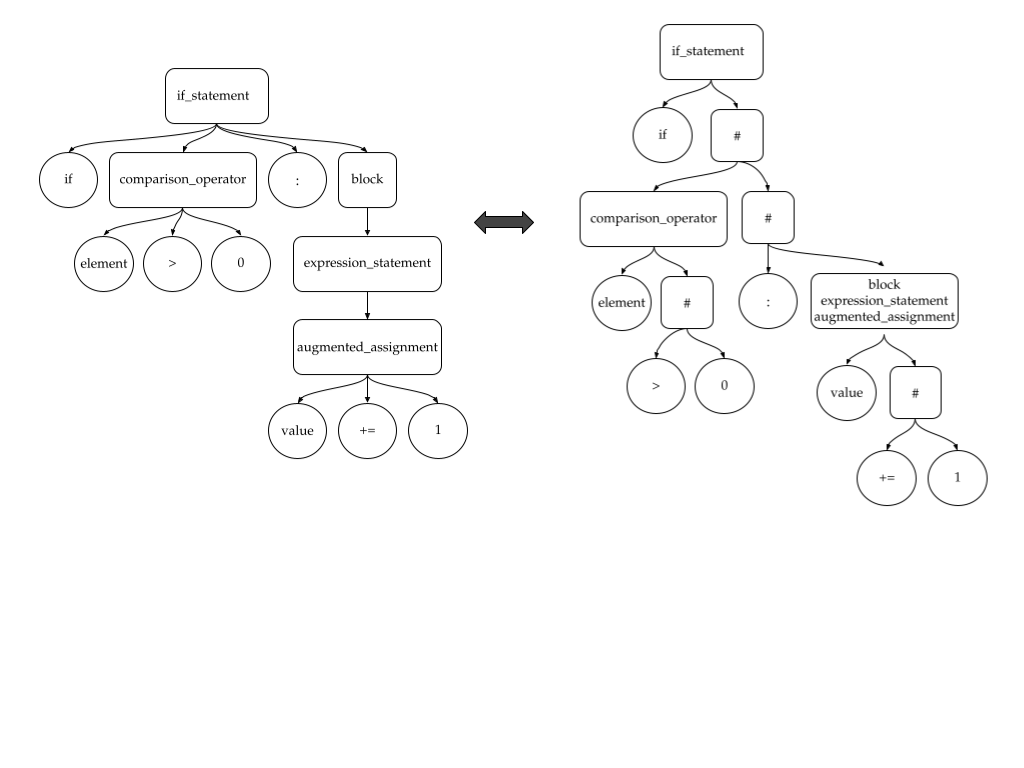
\includegraphics[width=\textwidth]{figures/ast-bt.png}
    \vspace{-130pt}
    \caption{Mapping an abstract syntax tree to its corresponding binary tree}
    \label{fig:ast-bt-mapping}
\end{figure}

For inference, one such trained NMT model can be leveraged to predict the linearized binary tree representation of the partial program under study.
The linearized binary tree representation can be used to reconstruct a unique binary tree (because of the one-to-one correspondence between them), and consequently the AST of the partial program. Moreover, the syntactic token types give information about a code token and its neighbors. Therefore, we plan to carry out both tasks, i.e., {\em syntactic-type tagging} and {\em partial AST-building} as a joint-learning process, which will help avoid error propagation from the former to the latter while benefiting each other. In addition, we will modify the decoding step in the NMT task to ensure that the ASTs thus generated for the partial programs are syntactically valid.
